\section{Prefix-free Code}
\begin{theorem}
Kraft Inequality: Every \textbf{prefix-free code} for an alphabet $\mathcal{X}$ with lengths $l(x)$ satisfies
$$\sum_{x\in\mathcal{X}}2^{-l(x)}\leq 1$$
当且仅当长度取到最优时等号成立. (i.e. $l(x)=\log\dfrac{1}{p_X(x)}$, $l(x)$为整数)
\end{theorem}

Proof: 将所有codebook中的 $01$ binary sequence 转成数字:
$$(0.c(x))=\left(0.y_1\ldots y_l\right)_2\to \left(\sum\limits_{m=1}^ly_m2^{-m}\right)_{10}\in[0,1)$$
Prefix-free 可以保证不存在 $\left(y_1\ldots y_l000\cdots\right)\sim\left(y_1\ldots y_l111\cdots\right)$ 之间的所有情况. 这个区间的code转换成的数字对应范围为
$$\left[\sum_{m=1}^ly_m2^{-m},\sum_{m=1}^ly_m2^{-m}+\sum_{i=l+1}^{+\infty}2^{-i}\right)=\left[\sum_{m=1}^ly_m2^{-m},\sum_{m=1}^ly_m2^{-m}+2^{-l}\right)$$
即占据一段长度为$2^{-l(x)}$的左闭右开的区间. prefix-free的code对应的区间必然没有overlap, 即
$$\sum_{x\in\mathcal{X}}2^{-l(x)}\leq 1$$

\begin{figure}[htbp]
    \centering
    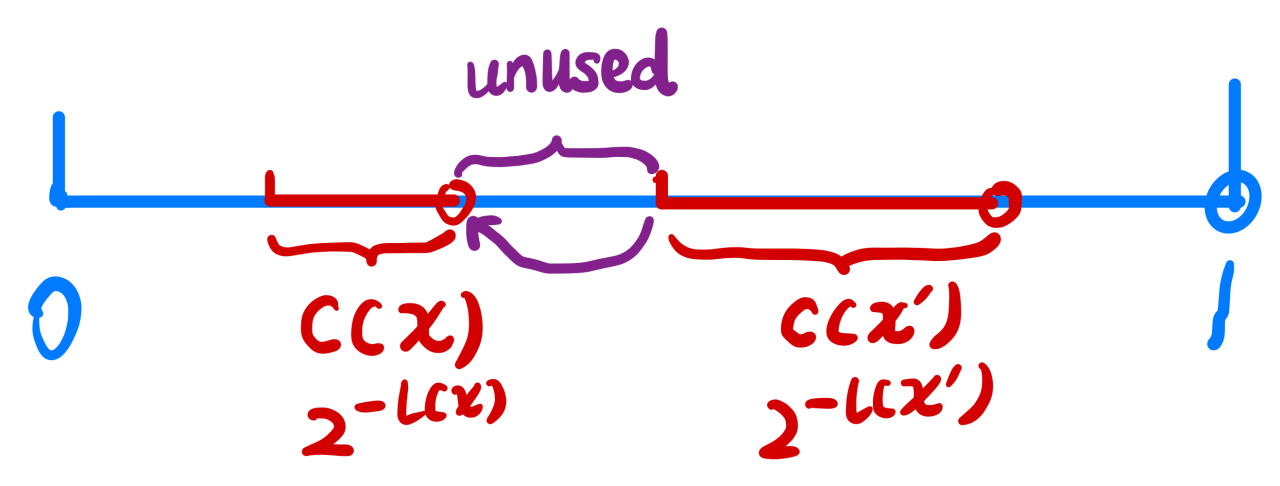
\includegraphics[width=0.8\textwidth]{./figures/chapter3/kraft_inequality.png}
\end{figure}

Optimal prefix-free code: 考虑优化问题, 先忽略码字长度必须为整数的限制:
\begin{align*}
\overline{L}_{\min} &= \min_{l_1,\ldots,l_M} \sum_{i=1}^M p_i l_i \\
s.t. &\qquad \sum_{i=1}^M 2^{-l_i} \leq 1
\end{align*}
Lagrange function
\begin{align*}
\mathcal{L}(l_1,\ldots,l_M,\lambda) &= \sum_{i=1}^M p_i l_i + \lambda \left(\sum_{i=1}^M 2^{-l_i} - 1\right) \\
\dfrac{\partial \mathcal{L}}{\partial l_i} = 0 &\Rightarrow p_i = \left(\lambda\ln 2\right) 2^{-l_i}
\end{align*}
因为我们想要让所有的$l_i$都尽可能小, 所以我们可以取Kraft不等式的等号, 并且将所有的$p_i = \left(\lambda\ln 2\right) 2^{-l_i}$相加可得
\begin{align*}
\sum_{i=1}^M p_i = 1 &= \lambda \ln 2 \sum_{i=1}^M 2^{-l_i} = \lambda \ln 2 \\
\Rightarrow \lambda &= \dfrac{1}{\ln 2} \\
\Rightarrow p_i &= 2^{-l_i}
\end{align*}
所以在忽略码字长度必须为整数的限制时, 最优的码字长度为$-\log p_i$, 且
$$\overline{L}_{\min} = \sum_{x}p(x)l(x)=\sum_{x}p(x)\log \dfrac{1}{p(x)} = H(X)$$
所以$H(X)$有了新的物理意义: 对 source code 进行压缩之后的最优期望码长.

现在考虑加上整数限制的情况:
\begin{theorem}
给定 DMS $X$, 则minimum expected codeword length for all prefix-free codes is
$$H(X)\leq \overline{L}_{\min}< H(X)+1$$
\end{theorem}
证明该定理: 只需要存在一种编码方式使得$\overline{L}_{\min}<H(X)+1$即可, 但是需要所有的编码方式都有 $H(X)\leq \overline{L}_{\min}$.

1. Shannon code: $l_i=\lceil\log \dfrac{1}{p_i}\rceil$, we have $\log\dfrac{1}{p_i}\leq l_i < \log\dfrac{1}{p_i}+1$, so
\begin{align*}
\overline{L}_{\min} &= \sum_{i=1}^M p_i l_i \\
&= \sum_{i=1}^M p_i \lceil\log \dfrac{1}{p_i}\rceil \\
&< \sum_{i=1}^M p_i \left(\log \dfrac{1}{p_i}+1\right) \\
&= \sum_{i=1}^M p_i \log \dfrac{1}{p_i} + \sum_{i=1}^M p_i \\
&= H(X)+1
\end{align*}
2. 考虑所有情况:
\begin{align*}
H(X) - \overline{L}_{\min} &= \sum_{i=1}^M p_i \log \dfrac{1}{p_i} - \sum_{i=1}^M p_i l_i = \sum_{i=1}^M p_i \log \left(\dfrac{2^{-l_i}}{p_i}\right) \\
&\leq \log\left(\sum_{i=1}^M p_i \dfrac{2^{-l_i}}{p_i}\right) \text{\qquad (Jensen's inequality, $\log x$ is concave)} \\
&= \log\left(\sum_{i=1}^M2^{-l_i}\right) \\
&\leq \log 1 \text{\qquad\qquad\qquad\quad\ \ (Kraft inequality)} \\
&= 0
\end{align*}
取等条件: \\
1. Jensen's Inequality: $2^{-l_i}=p_i$ (无法人为控制). \\
2. Kraft inequality: $\sum\limits_{i=1}^M2^{-l_i}=1$ (可以通过调整编码方式来尽可能的控制). \\
block-coding: $l_i=\log\dfrac{1}{p_i}\Rightarrow l_i=\log\left(\dfrac{1}{p_i}\right)^n=\dfrac{1}{n}\log\dfrac{1}{p_i}$ \\
可以渐进逼近最优(Jensen's inequality取等), 但codebook 复杂度指数级增加.